\chapter{\label{The CMS detector}The CMS detector}
The 27-km Large Hadron Collider (LHC) is the largest and most powerful particle accelerator ever built. It accelerates protons to nearly the velocity of light -- in clockwise and anti-clockwise directions -- and then collides them at four separate locations around its ring as shown in the \autoref{fig:my_label_LHC}. At these points, the energy of the particle collisions gets transformed into mass, spraying particles in all directions (\url{https://cms.cern/detector}).
% This will help us answer questions such as: "what is the Universe really made of and what forces act within it?" and "what gives everything substance?" Such research increases our basic understanding and may also spark new technologies that change the world we live in.\\
The Compact Muon Solenoid (or CMS) detector located at one of these four collision points. It is designed to observe any new physics phenomena that the LHC might reveal.CMS acts as a giant, high-speed camera, taking 3D “photographs” of particle collisions from all directions up to 40 million times per second. Although most of the particles produced in the collisions are “unstable” and short-lived, they transform rapidly into stable particles which can be detected by CMS.\\
 CMS is 15 meters in diameter. The CMS magnet is the central device around which the experiment is built, with a 4 Tesla magnetic field that is nearly $10^6$ times stronger than the Earth’s.(\url{https://cms.cern/detector/bending-particles})
 \begin{figure}[H]
     \centering
     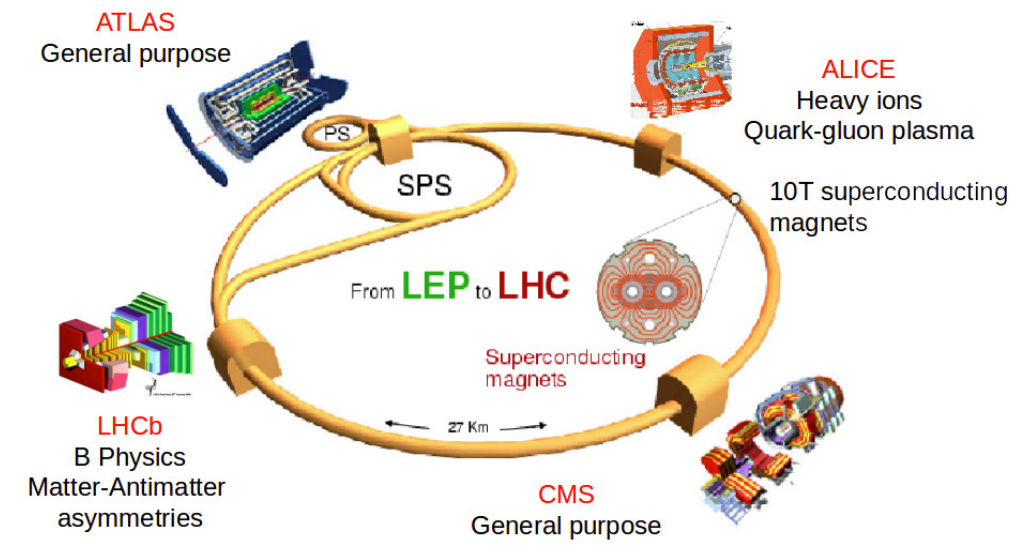
\includegraphics[scale=0.3]{14__ml.png}
     \caption{LHC}
     \label{fig:my_label_LHC}
 \end{figure}
As we know, higher the energy of the particle, the greater the amount of material needed to track. Similarly, to measure the momentum of a particle we track its path with the help of magnetic field, as greater the momentum the less it bends within it.
\url{https://cms.cern/detector}\\



The more momentum a particle has the less possibility of its path may get curved by the magnetic field, so tracing its path gives a measure of momentum of the particles. The tracker and calorimeter detectors (ECAL and HCAL) fit snugly inside the magnet coil whilst the muon detectors are inserted with a 12-sided iron structure that surrounds the magnet coils and contains and guides the field(as can be seen from the \autoref{fig:my_label_detect}).[\url{https://cms.cern/detector/bending-particles}]
The main function of CMS:
\begin{itemize}
    \item Bending Particles
    \item Identifying tracks
    \item Measuring energy
    \item Detecting muons
\end{itemize}
There are many other use such as medical imagining and etc.\\

 CMS consists of layers of detector material that exploit the different properties of particles to catch and measure the energy or momentum of each one. New particles discovered in CMS will be typically unstable and rapidly transform into a cascade of lighter, more stable and better-understood particles

\begin{figure}[h]
    \centering
    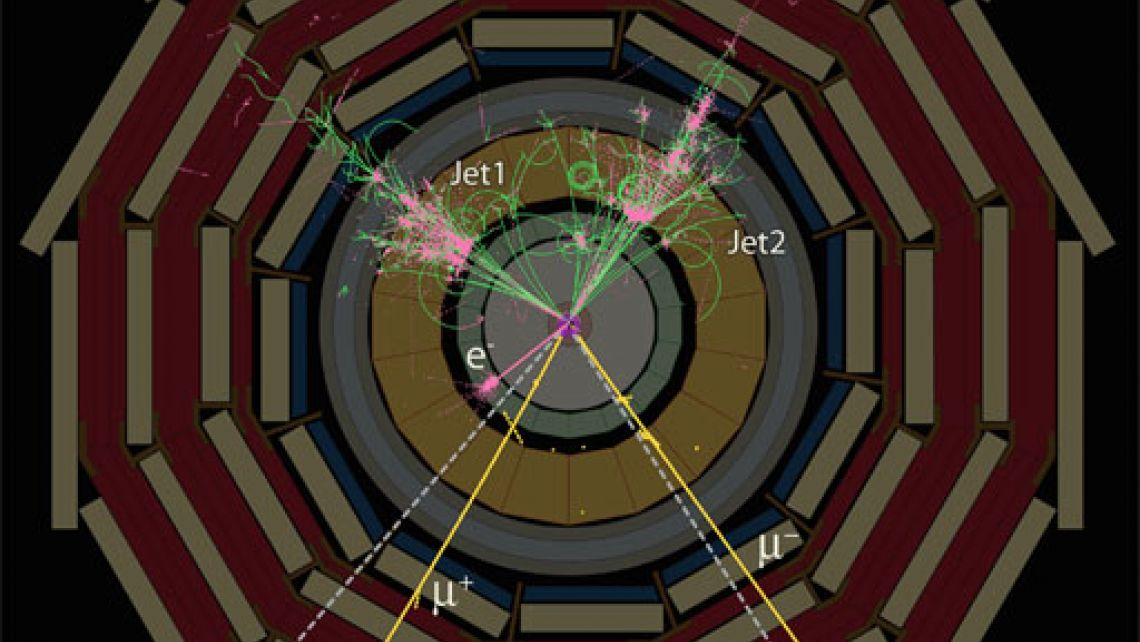
\includegraphics[scale=0.3]{Figures/SusyAny.jpg}
    \caption{This event shows the production of a supersymmetric particle. The decay of the particle is such that every single layer of CMS is needed to detect the full range of emerging particles: electrons, muons, neutrinos and jets, produced by quarks.[Source: \url{https://cms.cern/news/how-cms-detects-particles}]}
    \label{fig:my_label}
\end{figure}


% \includemovie{1cm}{1cm}{Figures/detectoroverview.gif}
% \includegraphics{Figures/detectoroverview.gif}
A particle which emerges from the collision, travel outwards will first encounter the tracking system, made of silicon pixels and silicon strip detectors. This pixels and strip detectors act as a camera. These accurately measure the positions of passing charged particles and allowing physicists to reconstruct their tracks. Charged particles follow spiraling paths in the CMS magnetic field and the curvature of their paths reveal their momenta.[\url{https://cms.cern/news/how-cms-detects-particles}]\\
The energies of the emerged particles will be measured in the next layer of the detector, the so-called calorimeters. Electrons, photons and jets (sprays of particles produced by quarks) will all be stopped by the calorimeters, allowing their energy to be measured.The first calorimeter layer is designed to measure the energies of electrons and photons with great precision. Since these particles interact electromagnetically, it is called an electromagnetic calorimeter (ECAL).[\url{https://cms.cern/detector/measuring-energy}]\\
Particles that interact by the strong force, hadrons, deposit most of their energy in the subsequwnt layer, the hadronic calorimeter (HCAL). The only known particles to penetrate beyond the HCAL are muons and weakly interacting particles such as neutrinos. Muons are charged particles, which are then tracked further in muon chamber detectors. Their momenta are also measured from the bending of paths in the CMS magnetic field. Neutrinos, however, are neutral and since they hardly interact at all they will escape detection.By adding up the momenta of all the detected particles, and assigning the missing momentum to the neutrinos, we can tell where these particles were.\\

% \section{TRIGGERING AND DATA ACQUISITION}
We need a "trigger" to select the potentially interesting events (such as Higgs particle) from larger amount of data produces after collision of proton-proton interaction. These trigger helps to reduce the rate to just a few hundred “events” per second, which can be read out and stored on computer disk for subsequent analysis. At the end, We are only left with only the collision events that might teach us something new about physics.[\url{https://cms.cern/detector/triggering-and-data-acquisition}]\\ 
% When CMS is performing at its peak, about one billion proton-proton interactions will take place every second inside the detector. There is no way that data from all these events could be read out, and even if they could, most would be less likely to reveal new phenomena; they might be low-energy glancing collisions for instance, rather than energetic, head-on interactions.We therefore need a “trigger” that can select the potentially interesting events, such as those which will produce the Higgs particle, and reduce the rate to just a few hundred “events” per second, which can be read out and stored on computer disk for subsequent analysis.\\

% However, with groups of protons colliding 40 million times per second there are only ever 25 nanoseconds (25 billionths of a second) before the next lot arrive. New waves of particles are being generated before those from the last event have even left the detector! The solution is to store the data in pipelines that can retain and process information from many interactions at the same time. To not confuse particles from two different events, the detectors must have very good time resolution and the signals from the millions of electronic channels must be synchronised so that they can all be identified as being from the same event.\\
% Level 1 of the trigger is an extremely fast and wholly automatic process that looks for simple signs of interesting physics, e.g. particles with a large amount of energy or in unusual combinations. This is like a reader simply scanning the headlines of a newspaper to see if anything catches their eye. This way we select the best 100,000 events or “issues” each second from the billion available. For the next test, the higher level trigger, we assimilate and synchronise information from different parts of the detector to recreate the entire event - like collating the different pages to form the full newspaper - and send it to a farm of more than 1000 standard computers.


% \url{https://cms.cern/detector/triggering-and-data-acquisition}


% \section{SILICON STRIPS}
% https://cms.cern/detector/identifying-tracks/silicon-strips
On the way out of the tracker, particles pass through ten layers of silicon strip detector of 130 centimeters.This tracker silicon strip detector consists of four inner barrel (TIB) layers assembled in shells with two inner endcaps (TID), each with three small discs. The outer barrel (TOB) consists of six concentric layers( as seen in \autoref{}). Finally two endcaps (TEC) close off the tracker. Each has silicon modules designed differently for its place within the detector. This part of the tracker contains 15,200 highly sensitive modules with a total of 10 million detector strips read by 80,000 microelectronic chips. Each module consists of three elements: sensors, mechanical support structure and electronics. These silicon are very suited to receive many particles in a small space due to their fast response and good spatial resolution. The small amount of charge generated after knocking of electron from atoms get amplified by APV25 chips, allows us to reconstruct its path.


\begin{figure}[H]
    \centering
    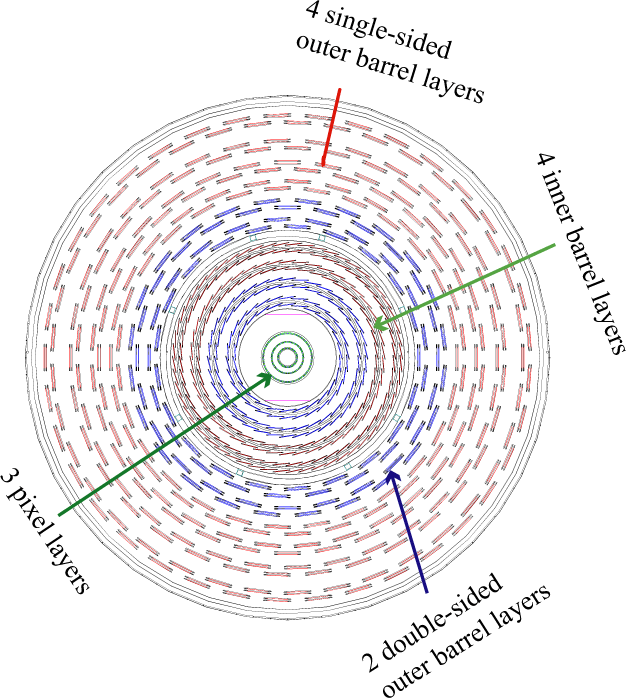
\includegraphics[scale=0.5]{Barrel.png}
    \caption{CMS Tracker layer shown in perpendicular to the beam[Source:\url{https://cms.cern/detector/identifying-tracks/silicon-strips}]}
    \label{fig:my_label}
\end{figure}


% After the pixels and on their way out of the tracker, particles pass through ten layers of silicon strip detectors, reaching out to a radius of 130 centimetres.
% The tracker silicon strip detector consists of four inner barrel (TIB) layers assembled in shells with two inner endcaps (TID), each composed of three small discs. The outer barrel (TOB) consists of six concentric layers. Finally two endcaps (TEC) close off the tracker. Each has silicon modules designed differently for its place within the detector. This part of the tracker contains 15,200 highly sensitive modules with a total of 10 million detector strips read by 80,000.  Each module consists of three elements: a set of sensors, its mechanical support structure and readout electronics. \\
% Silicon sensors are highly suited to receive many particles in a small space due to their fast response and good spatial resolution. microelectronic chips. Each module consists of three elements: a set of sensors, its mechanical support structure and readout electronics. \\
% Silicon sensors are highly suited to receive many particles in a small space due to their fast response and good spatial resolution. The silicon detectors work in much the same way as the pixels: as a charged particle crosses the material it knocks electron from atoms and within the applied electric field these move giving a very small pulse of current lasting a few nanoseconds. This small amount of charge is then amplified by APV25 chips, giving us “hits” when a particle passes, allowing us to reconstruct its path.

% Due to the nature of their job, the tracker and its electronics are pummeled by radiation but they are designed to withstand it. To minimise disorder in the silicon this part of the detector is kept at -20oC, to “freeze” any damage and prevent it from perpetuating.

% The charge on each microstrip is read out and amplified by an Analogue Pipeline Voltage (APV25) chip. Four or six such chips are housed within a “hybrid”, which also contains electronics to monitor key sensor information, such as temperature, and provide timing information in order to match “hits” with collisions. The APV25 stores the signals in a memory for several microseconds and then processes them before sending to a laser to be converted into infrared pulses. These are then transmitted over a 100m fibre optic cable for analysis in a radiation-free environment. The tracker uses 40,000 such fibre optic links providing a low power, lightweight way of transporting the signal. Much of the technology behind the tracker electronics came from innovation in collaboration with industry. \\
% \section{SILICON PIXELS}

% https://cms.cern/detector/identifying-tracks/silicon-pixels

% \section{TRACKING}
% https://cms.cern/detector/identifying-tracks

% The pixel detector, though about the size of a shoebox, contains 65 million pixels, allowing it to track the paths of particles emerging from the collision with extreme accuracy. Each layer is spilt into segments like tiny kitchen tiles, each a little silicon sensor, 100µm by 150µm, about two hairs widths. When a charged particle passes through it gives enough energy for electrons to be ejected from the silicon atoms, creating electron-hole pairs. Each pixel uses an electric current to collect these charges on the surface as a small electric signal. A electronic silicon chip, one for each tile is attached, using an almost microscopic spot of solder using the so-called bump bonding technique, which amplifies the signal.Knowing which pixels have been touched allows us to deduce the particle's trajectory. And because the detector is made of 2D tiles, rather than strips, and has a number of layers, we can create a three-dimensional picture. Because there are 65 million channels, the power for each pixel must be kept to a minimum. Even with each only generating around 50 microwatts, the total power output is around the same as the energy produced by a hot plate. So as not to overheat the detector, the pixels are mounted on cooling tubes.\\
% % \section{MEASURING ENERGY}
% https://cms.cern/detector/measuring-energy
The Electromagnetic Calorimeter (ECAL) is the inner layer of the two and measures the energy of electrons and photons by stopping them completely. Hadrons, which are composite particles made up of quarks and gluons, fly through the ECAL and are stopped by the outer layer called the Hadron Calorimeter (HCAL). Photodetectors that have been especially designed to work within the high magnetic field, are also glued onto the back of each of the crystals to detect the scintillation light and convert it to an electrical signal.
 
% \section{ENERGY OF ELECTRONS AND PHOTONS (ECAL)}
% https://cms.cern/detector/measuring-energy/energy-electrons-and-photons-ecal\\
% CMS must find the energies of emerging particles. Of particular interest are electrons and photons, because of their use in finding the Higgs boson and other new physics.

% The particles are measured using an electromagnetic calorimeter (ECAL). But to find them with the necessary precision in the very strict conditions of the LHC - a high magnetic field, high levels of radiation and only 25 nanoseconds between collisions - required very particular detector materials.\\ 
% Lead tungstate crystal is made primarily of metal and is heavier than stainless steel, but with a touch of oxygen in this crystalline form it is highly transparent and “ scintillates ” when electrons and photons pass through it. This means it produces light in proportion to the particle’s energy. These high-density crystals produce light in fast, short, well-defined photon bursts that allow for a precise, fast and fairly compact detector.

% Photodetectors that have been especially designed to work within the high magnetic field, are also glued onto the back of each of the crystals to detect the scintillation light and convert it to an electrical signal that is amplified and sent for analysis.

% The ECAL, made up of a barrel section and two ”endcaps”, forms a layer between the tracker and the HCAL. The cylindrical “barrel” consists of 61,200 crystals formed into 36 “supermodules”, each weighing around three tonnes and containing 1700 crystals. The flat ECAL endcaps seal off the barrel at either end and are made up of almost 15,000 further crystals.

% For extra spatial precision, the ECAL also contains Preshower detectors that sit in front of the endcaps. These allow CMS to distinguish between single high-energy photons (often signs of exciting physics) and the less interesting close pairs of low-energy photons.
% The CMS ECAL…

% crystals each weigh 1.5kg but with a volume roughly equal to that of a small coffee cup,
% contains nearly 80,000 such crystals, each of which took two days to grow.

% https://cms.cern/detector/measuring-energy/energy-hadrons-hcal\\

% https://cms.cern/detector/detecting-muons\\
% https://cms.cern/detector/computing-grid\\
A huge amount of data, obtained from CMS that must be analysed, and to meet this challenge, the LHC employs a novel computing system, a distributed computing and data storage infrastructure called the Worldwide LHC Computing Grid (WLCG). In ‘The Grid’, tens of thousands of standard PCs collaborate worldwide to have much more processing capacity than could be achieved by a single supercomputer, giving access to data to thousands of scientists all over the world.\url{https://cms.cern/detector/computing-grid}

% The “Tier 0” centre at CERN first reconstructs the full collision events and analysts start to look for patterns; but the data has a long way to go yet. Once CERN has made a primary backup of the data it is then sent to large “Tier 1” computer centres in seven locations around the world: in France, Germany, Italy, Spain, Taiwan, the UK and the US. Here events are reconstructed again, using information from the experiment to improve calculations using refined calibration constants.

% Tier 1 starts to interpret and make sense of the particle events and collate the results to see patterns emerging. Meanwhile each sends the most complex events to a number of “Tier 2” facilities, which total around 40, for further specific analysis tasks. In this way information braches out from each tier across the world so that, on a local level.
% , physicists and students whether in Rio de Janeiro or Oxford, can study CMS data from their own computer, updated on a regular basis by the LHC Computing Grid.
 Charged particle trajectories are measured by the silicon pixel and strip sub detectors, covering 0 <$\phi$ <2$\pi$ in azimuth and $|\eta|$ < 2.5, where the pseudo rapidity $\eta$ is defined as 
 \begin{equation*}
     \eta = -ln[\tan \theta/2],
 \end{equation*}
 
 with $\theta$ being the polar angle of the trajectory of the particle with respect to the counterclockwise-beam direction. Within the field
volume, the silicon detectors are surrounded by a crystal electromagnetic calorimeter and a brass/scintillator hadron calorimeter that provide high resolution energy measurement of photons, electrons and hadronic jets.

\setcounter{equation}{0}
\setcounter{table}{0}
\setcounter{figure}{0}
%\baselineskip 24pt


    



